\documentclass[a4paper, titlepage, final]{article}
\usepackage{ngerman, dramatist, adjmulticol, lipsum, type1cm, lettrine, graphicx}
\usepackage[pdftex,bookmarks=true]{hyperref}
\author{Fabio Madge-Pimentel\\
	Josef-Hofmiller Gymnasium Freising, 10b\\
	\texttt{fabio@madge.me}}
\title{Lesetagebuch zu Schillers Drama "`Die R"auber"'}
\date{31. Januar 2012}
\pagenumbering{arabic}
\pagestyle{headings}

\begin{document}

\maketitle

\tableofcontents
\newpage

\part{Personenregister}
	\paragraph{Maximilian}
Altersm"uder, leichtgl"aubiger Mann, ohne gro"se Ambitionen
\paragraph{Karl}
Junger st"urmischer Mann, gutaussehend und intelligent
\paragraph{Franz}
K"uhler, schlecht aussehender Taktiker ohne Ideale
\paragraph{Amalia von Edelreich}
Treu Liebende, attraktive junge Frau
\paragraph{Libertiner}
Gruppe ergebender R"auber, deren Lebensmittelpunkt die Bande bildet
\subparagraph{Spiegelberg}
Gegenspieler Karls, der keinen Verbrechen f"urchtet
\paragraph{Daniel}
Alter, treuer Hausangestellter
\paragraph{Hermann}
Leicht beeinflussbarer, aber im Herzen guter Mann
\paragraph{Pastor Moser}
"Uberlegter Kleriker
\newpage
\part{Karl von Moor}
	\section{Charakterisierung}
		Karl Moor ist der "alteste Sohn des alten Moor und steht seit seiner Kindheit mit seinem Bruder Franz in Rivalität um die Gunst dessen, wobei Karl generell im Vorteil lieg. Dies ist zum einen durch seinen guten "au"seren Qualitäten, aber auch seinen Intellekt bedingt.
Zu Beginn des Dramas ist er als Student in Leipzig, bricht sein Studium jedoch, wegen der Entt"auschung "uber die Versto"sung des Vaters, zugunsten einer Karriere als R"auber ab. In dieser Profession bek"ampft er als Hauptmann einer R"aberbande die Ungerechtigkeiten im Staat, kann sich jedoch zu keinem Zeitpunkt von seiner Liebe Amalia l"osen.
%	\newpage
	\section{Steckbrief}
		\begin{center}
\begin{huge}
\textbf{\uppercase{Steckbrief}}
\end{huge}
\end{center}

\begin{center}
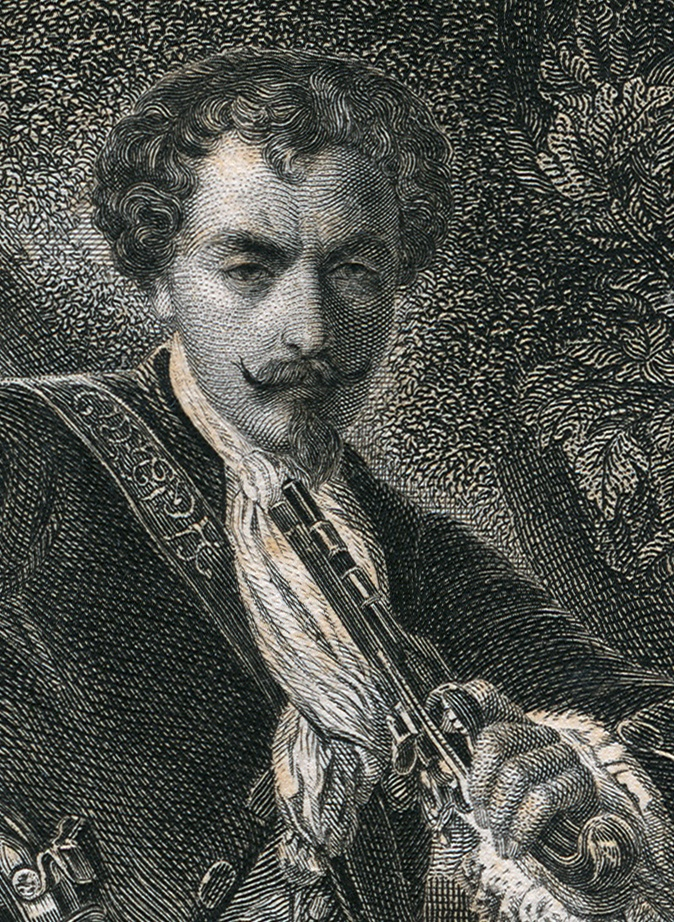
\includegraphics[scale=2.5]{karl}
\end{center}

\begin{center}
Der hier gezeigte  R"auberhauptmann \textbf{\uppercase{Karl von Moor}} wird aufgrund diverser Vergehen gegen die Menschlichkeit gesucht. Dem Finder werden
\end{center}

\begin{center}
\begin{huge}
\textbf{1000} Louis d'or
\end{huge}
\end{center}

\begin{center}
geboten. Der Gesuchte ist etwa \textbf{29 Jahre} alt und etwa \textbf{6 Schuh} gro"s.
\end{center}
\newpage
\part{Textarbeit}
	\section{Schaupl"atze}
		\paragraph{Das Moorsche Schloss}
Saal, Amaliens Zimmer, Moors Zimmer, Schlossgarten, Galerie, Anderes Zimmer
\paragraph{Schenke an den Grenzen von Sachsen}
Lauter Tolle Sachen
\paragraph{Die b"omischen W"alder}
Echt Tolle Sachen
\paragraph{Gegend an der Donau}
R"auber auf einem von B"aumen geschützen H"ugel, die Pferde unten am Weiden.
\paragraph{Um das Schloss}
L"andlieche Gegend in der Umgebung, Schloss im Wald
	\section{Regiebuch}
		\Character[MAXIMILIAN, regierender Graf von Moor]{Der alte Moor}{moor}
\Character[FRANZ, sein Sohn.]{Franz}{fran}

\begin{center}

\Large{Erster Akt}

\large{Erste Szene}

\end{center}

\StageDir{Franken. Saal im Moorschen Schloss.\\
	\fran: Betritt den Raum mit der Hand in der Innentasche [Zufrieden, aber gegenteiliges Verhalten nach au"sen]\\
	\moor: Schwach, Gequ"alt; Position: Im Thron; Blick: nach drau"sen}

[...]

\begin{drama}

\franspeaks \direct{nimmt den Brief aus der Tasche.} Ihr kennt unsern Korrespondenten! Seht! Den Finger meiner rechten Hand wollt' ich drum geben, d"urft ich sagen, er ist ein L"ugner, ein schwarzer giftiger L"ugner --- Fasst Euch! Ihr vergebt mir, wenn ich Euch den Brief nicht selbst lesen lasse -- Noch d"orft Ihr nicht alles h"oren.
\moorspeaks \direct{l"asst sich weiter sacken.} Alles, alles -- mein Sohn, du ersparst mir die Kr"ucke.
\franspeaks \direct{kommt n"aher und liest.} \frqq Leipzig, vom 1. May. -- Verb"ande mich nicht eine unverbr"uchliche Zusage, dir auch nicht das geringste zu verhehlen, was ich von den Schicksalen deines Bruders auffangen kann, liebster Freund, nimmermehr w"urde meine unschuldige Feder an dir zur Tyrannin geworden sein. Ich kann es aus hundert Briefen von dir abnehmen, wie Nachrichten dieser Art dein br"uderliches Herz durchbohren m"u"sen, mir ist's als s"ah ich dich schon um den Nichtsw"urdigen, den Abscheulichen\flqq \ --- \direct{Der alte Moor verbirgt sein Gesicht.} Seht, Vater! ich lese Euch nur das glimpflichste -- \frqq den Abscheulichen in tausend Thr"anen ergossen\flqq , ach, sie flossen -- st"urzten stromweis von dieser mitleidigen Wange -- \frqq mir ist's, als s"ah ich schon deinen alten, frommen Vater totenbleich\flqq \ -- Jesus Maria! Ihr seid's, eh Ihr noch das Mindeste wisset?
\moorspeaks \direct{hebt seinen Kopf.} Weiter! Weiter!

\franspeaks \direct{n"ahert sich weiter.} \frqq Totenbleich in seinen Stuhl zur"ucktaumeln und dem Tage fluchen an dem ihm zum ersten Mal \emph{Vater} entgegengestammelt ward. Man hat mir nicht alles entdecken m"ogen, und von dem wenigen das ich weis erf"ahrst du nur weniges. Dein Bruder scheint nun das Ma"s seiner Schande gef"ullt zu haben; ich wenigstens kenne nichts "uber dem was er wirklich erreicht hat, wenn nicht sein Genie das meinige hierin "ubersteigt. Gestern um Mitternacht hatte er den gro"sen Entschlu"s, nach vierzig tausend Dukaten Schulden\flqq \ -- \direct{formt einen angewiderten Gesichtsausdruck und holt 40000 Dukaten aus seiner Tasche heraus.} ein h"ubsches Taschengeld Vater -- \frqq nachdem er zuvor die Tochter eines reichen Bankiers allhier entjungfert, und ihren Galan einen braven Jungen von Stand im Duell auf den Tod verwundet mit sieben andern, die er mit in sein Luderleben gezogen dem Arm der Justiz zu entlaufen\flqq \ -- Vater! Um Gotteswillen Vater! wie wird Euch?
\moorspeaks Es ist genug. -- La"s ab mein Sohn!

\end{drama}

[...]

\endinput
	\section{Neuformulierung}
		\Character[MAXIMILIAN, regiereder Graf von Moor]{Der alte Moor}{moor}
\Character[FRANZ, sein Sohn.]{Franz}{fran}

\begin{center}

\Large{Erster Akt}

\large{Erste Szene}

\end{center}

\StageDir{Franken. Saal im Schloss des alten Moors.\\\fran, \moor}

[...]

%mir ist’s als sa ̈h ich dich schon um den Nichtswu ̈rdigen, den Abscheulichen in tausend Thra ̈nen ergossen mir ists, als sa ̈h ich schon dei- nen alten, frommen Vater Todtenbleich

%Dich male ich mir schon aus, wie du um diesen Unw"urdigen, den Taugenichts weinst und deinen Vater dem Tode nahe

\begin{drama}

\franspeaks \direct{nimmt den Brief aus der Tasche.} Dir ist unser Korrespondent bekannt! Schau! Alles w"urde ich geben, k"o"nnte ich dir sagen, dass er ein L"ugner, ein dreckiger L"ugner, ist --- Beruhige dich! Du wirst mir nachsehen, dass ich dich den Brief nicht selbst lesen lasse -- Noch darfst du nicht alles h"oren.
\moorspeaks Alles, alles -- mein Sohn, du bist mir eine Hilfe.
\franspeaks \direct{liest.} \frqq Leipzig, vom 1. Mai. -- H"atte ich dir nicht versprochen dir nichts, das Schicksal deines Bruders betrefflich, zu verschweigen, mein Freund, w"are ich der "Ubersendung des Folgenden aus dem Weg gegangen. Aus unseren vorhergegangenen Korrespondenzen schlie"se ich, wie sehr dich diese Nachricht qu"alen muss. Dich male ich mir schon aus, wie du um diesen Unw"urdigen, den Taugenichts\flqq \ --- \direct{Der alte Moor verbirgt sein Gesicht.} Schau, Vater! ich lese dir nur das schonendste vor -- \frqq den Taugenichts weinst\flqq , ja, sie haben mich ergriffen -- haben mich eingenommen -- \frqq und deinen Vater dem Tode nahe\flqq \ -- Oh Gott! Ich sehe dich diesem Zustand schon so nahe, doch hast du noch nichts erfahren.
\moorspeaks Weiter! Weiter!

\end{drama}

[...]

\endinput
\newpage
\part{Freiarbeit}
	\section{Beurteilung}
		Mit seinem Werk "`Die R"auber"' bringt Schiller es fertig ein zeitloses Werk zu schaffen, welches trotz seines nicht zeitgem"a"sen Rahmens und der ebsenso zu bewertenden Sprache immernoch aktuell ist und auf unsere Zeit angewendet werden kann. Jedoch ist der literrarische Anspruch der seinen Themen entgegengebracht wurde in meinen Augen bewusst zu hoch angesetzt, was dazu f"uhrt, dass,  heute wie damals, Teile der Bevo"lkerung als Publikum ausgeschlossen werden.
	\section{Alternatives Ende}
		Phasellus dapibus, arcu ut facilisis fermentum, neque nisi ornare orci, sit amet vestibulum justo est id orci. Quisque luctus cursus enim sed imperdiet. In a velit eu ligula tristique eleifend eu quis magna. Ut id mauris vitae libero feugiat porttitor. Donec consequat nibh in neque placerat ultricies. Pellentesque blandit magna eget quam volutpat a volutpat neque congue. Nulla porttitor volutpat mi sit amet bibendum. Sed congue mollis imperdiet. Suspendisse tincidunt hendrerit placerat. In ut leo quam, ut vehicula purus.

Sed imperdiet libero vel nunc placerat vel varius massa rhoncus. Pellentesque habitant morbi tristique senectus et netus et malesuada fames ac turpis egestas. Sed augue turpis, consectetur id vestibulum id, dignissim sed neque. Quisque scelerisque iaculis felis, in condimentum nisl bibendum non. Maecenas velit mi, molestie sit amet ultrices sit amet, lobortis a leo. Nulla facilisi. Nunc fringilla sollicitudin faucibus. Vivamus a nibh mi. Nulla gravida dolor sapien, eu tincidunt nunc. Cum sociis natoque penatibus et magnis dis parturient montes, nascetur ridiculus mus. Nunc odio nisl, vestibulum non fringilla ut, tempor eu nunc. Mauris porta, enim at hendrerit cursus, neque quam rutrum sapien, vel pellentesque mauris ligula eget nisl. Curabitur cursus, leo in gravida porttitor, libero eros auctor justo, tristique pretium magna augue eu metus.
	\section{Zeitungsbericht "uber die R"auber}
		\texttt{\Huge Gefahr aus dem Wald}
	\newline
\textit{\Large Die ersch"utternden Wahrheiten}
\normalsize

\begin{adjmulticols*}{3}{0pt}{0in}
 	\lettrine{W}{ie} jeder unserer treuen Leser bereits wei"s, treibt seit l"angerer Zeit eine R"auberbande in unseren Gefilden ihr Unwesen. Dabei geht sie zutiefst brutal vor und schreckt auch vor Menschenopfern nicht zur"uck.
 	Da der Umstand, dass "uber diese "Ubelt"ater nichts bekannt ist unsere Leser nachts nicht schlafen l"asst, haben wir unseren besten Mann auf die Spur dieser Ganoven gesetzt. Die Ergebnisse sind naturgem"a"s niederschmetternd.
 	Die Bande hat ihren Mittelpunkt in den b"omischen W"aldern gefunden, von dort starten sie ihre verh"angisvollen Streifz"uge. Als ihr Hauptmann konnte \textit{Karl von Moor} ausgemacht werden. Der entstammt dem Hause Moor, dessen alternder Vorsteher mit Ach und Krach versucht sein Land zu regieren.
 	Aber zum Gl"uck konneten wir auch Schachstellen ausmachen, so gibt es beispielsweise Probleme auf der F"uhrungsebene, dort m"ochte sich n"amlich auch \textit{Moritz Spiegelberg} positionieren.
 	Mehr k"onnen wir im Moment nicht berichten, aber "uber eins k"onnen sie versichert sein, wir verflogen diese Misset"ater f"ur sie weiter.
\end{adjmulticols*}		

\end{document}